\documentclass[10pt]{article}         %% What type of document you're writing.
\usepackage{graphicx}
\usepackage{hyperref}
\usepackage[dvipsnames]{xcolor}

%%%%% Preamble

%% Packages to use

\usepackage{amsmath,amsfonts,amssymb}   %% AMS mathematics macros

%% Title Information.

\title{Neural Network(alphabet katakana)}
\author{Leonardo Martinez}
%% \date{29 sep 2020}           %% By default, LaTeX uses the current date

%%%%% The Document

\begin{document}

\maketitle

\begin{abstract}
This document implements the neural network for the Japanese \\ alphabet (katakana).
\end{abstract}

\section{Introducción}
El presente proyecto esta diseñado para la realización de una red neuronal, la cual busca por medio de la implementación de cálculos matemáticos y \\programación en el lenguaje "C++" obtener la probabilidad de que un dato de entrada se asemeje con los datos previamente cargados para entrenar la red neuronal.\\
En esta ocasión esta red está pensada para el abecedario japones katakana, los datos de entrenamiento será el abecedario representado en matrices de 16*16 para un mejor resultado de aproximación.\\
Antes de pasar a la implementación de código ser realizará un prototipado con la herramienta matlab para verificación correcta de los cálculos matemáticos y así obtener los resultados esperados a la hora de ejecutar el programa.\\
\\
Para la realización el prototipado en matlab realizaremos matrices de 18 * 18 ya que al multiplicar tenemos como resultado 324 datos que al ocupar la formula que se nos proporciona en el libro (Multiplicar N por 0.15) obtenemos la cantidad minima para comparar, es decir, 324 * 0.15 = 48.6, dicho resultado es suficiente debido a que nuestro abecedario japones consta de 46 letras .   	

\begin{figure}[htb]
\centering
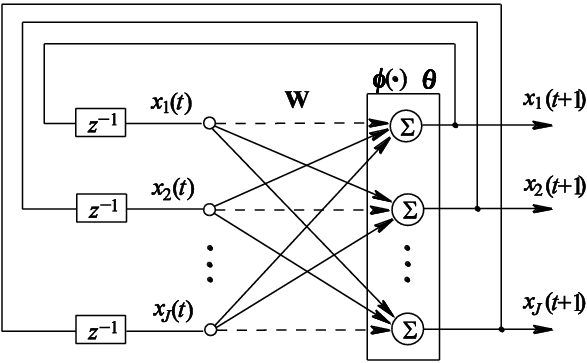
\includegraphics[width=0.5\textwidth]{hopfield.png}
\caption{Hopfield Model Neural Network}
\label{fig:tigre}
\end{figure}





\section{Desarrollo}



\section{Conclusión}


	

\end{document}
